\documentclass[12pt,a4paper]{article}

\usepackage[utf8]{inputenc}
\usepackage[T1]{fontenc}
\usepackage{lmodern}
\usepackage[margin=2.5cm]{geometry}
\usepackage{setspace}
\usepackage{microtype}
\usepackage{booktabs}
\usepackage{tabularx}
\usepackage{array}
\usepackage{amsmath,amssymb}
\usepackage{xcolor}
\usepackage{hyperref}
\usepackage{enumitem}
\usepackage[round,authoryear]{natbib}
\usepackage{tikz}
\usetikzlibrary{arrows.meta,positioning,shapes.geometric}

\definecolor{linkblue}{RGB}{25,82,140}
\definecolor{stageblue}{RGB}{235,243,250}
\definecolor{datagold}{RGB}{252,245,219}

\hypersetup{
  colorlinks=true,
  linkcolor=linkblue,
  citecolor=linkblue,
  urlcolor=linkblue,
  pdftitle={Direct Preference Optimisation for BioASQ Exact Answering}
}

\setlist{itemsep=0.3em,topsep=0.5em}
\renewcommand{\arraystretch}{1.15}
\onehalfspacing

\title{\textbf{Research Methodology Report}\\[0.6em]
\large Direct Preference Optimisation for BioASQ Exact Answering}
\author{}
\date{Activity 3 --- revised 5 October 2026}

\begin{document}

\maketitle


\section{Introduction}

BioASQ exact answering requires concise biomedical answers supported by scientific snippets. Factoid questions usually seek one entity or value, while list questions seek several distinct entities. Correctness depends on both identifying the requested concept and expressing it in an accepted form. Abbreviations, synonyms and alternative nomenclature can cause a scientifically correct answer to fail string-based evaluation. Improving this task therefore requires examining answer representation as well as biomedical reasoning \citep{tsatsaronis2015bioasq}.

This project investigates \textbf{whether Direct Preference Optimisation (DPO) improves BioASQ exact answering beyond supervised fine-tuning (SFT), and whether its effect changes under answer expansion and ranking}. The initial experiments trained single-output SFT models and subsequently applied DPO. The project reports that SFT improved BioASQ scores, whereas DPO provided only marginal additional benefit. This observation concerns the evaluated formulation and preference data; the present study tests whether a different output strategy creates more useful preference contrasts.

Two observations motivate that change. First, the Qwen2.5-3B SFT model achieved factoid MRR 0.44375 and LLM-judged semantic accuracy 0.8125 on 160 development questions; the corresponding 0.5B values were 0.40625 and 0.74375. For these single-answer outputs, MRR equals exact accuracy. The discrepancy suggests an answer-expression problem, although semantic judgments require auditing. Second, despite the larger model's higher aggregate score, some questions were correct only for the smaller model. Their complementary successes motivate combining outputs rather than assuming that model scale subsumes every smaller-model answer.

The revised strategy generates multiple evidence-supported candidates, combines model outputs and ranks the resulting pool. Promising coverage from expansion without additional BioASQ-specific training establishes a baseline for adaptation. A pool containing a gold answer does not guarantee that the system will rank it first: candidate recall and final answer quality must be evaluated separately.

The study addresses three questions:

\begin{enumerate}[label=\textbf{RQ\arabic*:}]
  \item What semantic, exact-form and cross-model errors remain after single-output SFT and DPO?
  \item Does controlled expansion and multi-model pooling improve candidate coverage and ranked exact answering over direct generation and repeated sampling?
  \item Does expansion SFT followed by DPO improve held-out exact-answer performance beyond expansion SFT alone, and through which changes in candidate quality?
\end{enumerate}

Factoid answering is the primary confirmatory task because its data and pilots are established. List answering is a planned secondary extension using the same comparisons with entity-set evaluation. Preference-trained selection is an optional diagnostic after the generator comparison. The expected contribution is evidence about where DPO adds value, supported by an analysis of answer-form errors and model complementarity. Small, absent or negative DPO effects remain informative research outcomes.

\section{Methodological Approach and Rationale}

\subsection{Experimental approach}

The project uses quantitative computational experiments with iterative system development. Preliminary observations identify failure modes; controlled interventions test whether changing output formulation and training addresses them. A \textbf{within-question paired design} supplies each method with identical questions and snippets. This controls question difficulty and evidence availability, allowing differences to be attributed more clearly to generation, pooling or adaptation.

The principal intervention is DPO after expansion SFT. Candidate recall is measured before ranking, and final scores are measured with selection held constant. This decomposition is necessary because a generator can increase coverage while also introducing incorrect candidates that make selection harder. It also avoids attributing a stronger selector's gains to generator DPO. Multi-model pools retain a fixed source composition and candidate budget across training conditions.

\subsection{Why expansion and ranking?}

Direct generation is a credible low-cost baseline, but one decoded answer commits to both a concept and an expression. Repeated stochastic generation provides alternatives without training; however, it may repeat the same answer and consumes additional requests. In the GPT-4.1-mini pilot, ten sampled responses covered 48.75\% of development questions, while one equivalent-expansion response covered 55.0\%. These are offline candidate-coverage results, not official ten-answer submissions. The comparison motivates explicit diversification, while token cost and matched candidate limits must still be controlled.

Literal extraction offers traceable evidence and limits unsupported reformulation. Nevertheless, the existing audit found a normalised gold-string occurrence in only 121 of 160 development questions. Absence of a literal alias does not establish absence of semantic support. Extraction is therefore retained as a grounded baseline, alongside equivalent-expression expansion. The latter can recover alternative names but can also change meaning. Evidence checks and semantic diagnostics are required rather than assuming every generated variant is valid.

Pooling is justified by complementary errors, not merely by using more models. The Llama-3.1-8B expansion pilot covered 52.5\% of questions, and its union with GPT-4.1 mini covered 63.75\%. Because that union can contain more candidates, unrestricted oracle coverage and fixed-budget pooled performance are reported separately. A supervised cross-encoder is a suitable ranking baseline because it jointly considers the question and candidate \citep{nogueira2019passage}; snippets are included to support evidence-sensitive selection.

\subsection{Why DPO rather than further SFT or reward-model-based optimisation?}

SFT teaches a target response; DPO uses preferred and rejected responses to adjust their relative likelihood against a reference policy \citep{rafailov2023dpo}. Here, comparisons can expose omitted accepted answers or unsupported variants that imitation alone may not explicitly contrast. Whether this signal helps BioASQ remains an empirical question.

Reward-model-based reinforcement learning is a reasonable alternative, but introduces a separately trained reward model and an online optimisation loop. DPO is selected for its simpler offline comparison pipeline \citep{rafailov2023dpo}, which fits the project's stored candidate banks and limited GPU allocation. This choice does not assume superior BioASQ accuracy. A continued-SFT control tests whether any gain instead comes from extra optimisation, while supervised reranking tests whether selection alone is sufficient.

QLoRA provides feasible adaptation of an 8B model through low-rank adapters and a frozen four-bit backbone \citep{dettmers2023qlora}. Its memory advantage enables controlled comparisons on available hardware, but conclusions will concern the evaluated quantised model. Expansion and DPO are thus selected for testability and resource fit, with their limitations measured explicitly.

\section{Research Design and Implementation}

\subsection{Data and separation}

The established factoid experiment contains 1,600 training-corpus questions, a fixed 160-question development set and a separate 95-question official test set. The confirmatory protocol retains the development set for diagnostic comparison and partitions the remaining 1,440 questions into 1,296 fitting and 144 internal-validation questions using sorted identifiers and seed 3407. All aliases, snippets, teacher targets and preferences inherit their question's partition. Lexical filtering applies only to fitting data; evaluation retains questions without extractable aliases.

The reused development set has already influenced design choices, so further hyperparameter selection uses internal validation. Test exposure will be audited before the final run. If a test batch has influenced previous choices, it will be labelled as previously inspected, and a new unseen batch will be reserved for confirmatory evaluation. Partition identifiers, exclusions and derived example counts will be saved in a manifest. Existing candidate banks are reusable for training only after their question membership is checked.

\subsection{Experimental sequence and controls}

The study proceeds through baseline diagnosis, candidate generation, pooling, matched adaptation and held-out scoring. Completed pilots motivate the design; the following conditions are proposed confirmatory experiments.

\begin{table}[htbp]
\centering
\caption{Matched generator comparisons.}
\label{tab:training}
\small
\setstretch{1.0}
\begin{tabularx}{\textwidth}{>{\raggedright\arraybackslash}p{0.12\textwidth}>{\raggedright\arraybackslash}X>{\raggedright\arraybackslash}X>{\raggedright\arraybackslash}X}
\toprule
\textbf{Condition} & \textbf{Generator} & \textbf{Selection held constant} & \textbf{Purpose} \\
\midrule
A & instruction-tuned checkpoint, without BioASQ adaptation & fixed ordering or frozen reranker & expansion baseline \\
B & expansion SFT & same as A & SFT increment \\
C & B followed by generator DPO & same as A & DPO increment beyond SFT \\
D & B with continued SFT & same as A & extra-optimisation control \\
\bottomrule
\end{tabularx}
\end{table}

Each condition is evaluated as an individual generator and within the same fixed-composition multi-model pool. In the pooled comparison, the focal model changes from A to B, C or D while the companion source remains frozen. This isolates adaptation from changes in model composition. Source-balanced round-robin ordering and a supervised reranker provide separate selection conditions; the reranker is trained once and frozen for all primary generator contrasts. Original single-output instruction-tuned, SFT and SFT-plus-DPO systems remain formulation controls.

\begin{figure}[htbp]
\centering
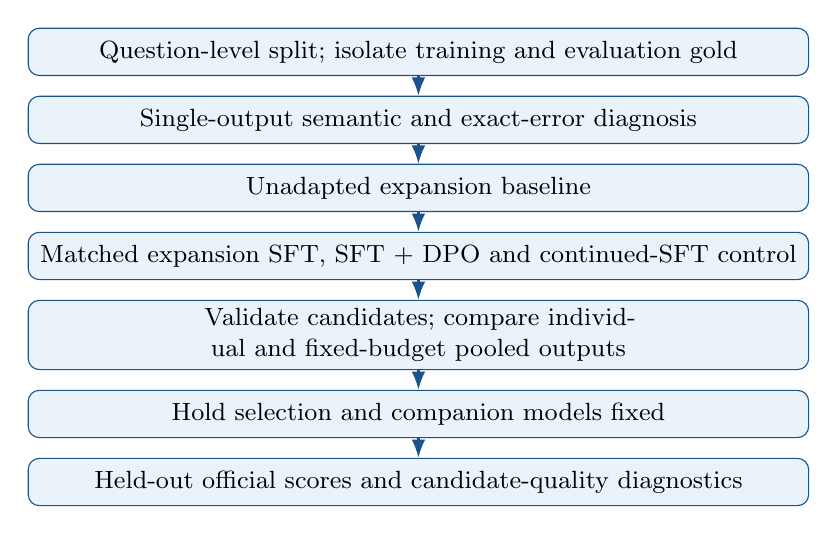
\begin{tikzpicture}[
  node distance=2.5mm,
  >=Latex,
  stage/.style={draw=linkblue,rounded corners,fill=stageblue,
    align=center,text width=0.80\textwidth,minimum height=6mm,
    inner sep=3pt,font=\small},
  flow/.style={->,thick,linkblue}
]
\node[stage] (split) {Question-level split; isolate training and evaluation gold};
\node[stage,below=of split] (diagnosis) {Single-output semantic and exact-error diagnosis};
\node[stage,below=of diagnosis] (baseline) {Unadapted expansion baseline};
\node[stage,below=of baseline] (training) {Matched expansion SFT, SFT + DPO and continued-SFT control};
\node[stage,below=of training] (pool) {Validate candidates; compare individual and fixed-budget pooled outputs};
\node[stage,below=of pool] (selection) {Hold selection and companion models fixed};
\node[stage,below=of selection] (evaluation) {Held-out official scores and candidate-quality diagnostics};
\draw[flow] (split) -- (diagnosis);
\draw[flow] (diagnosis) -- (baseline);
\draw[flow] (baseline) -- (training);
\draw[flow] (training) -- (pool);
\draw[flow] (pool) -- (selection);
\draw[flow] (selection) -- (evaluation);
\end{tikzpicture}
\caption{Experimental sequence. Gold answers supply training labels and offline
evaluation, but are excluded from development and test generation prompts.}
\label{fig:workflow}
\end{figure}

\subsection{Targets, preferences and ranking data}

Factoid expansion returns up to ten candidate strings with relation types and evidence provenance. The established prompt expands one inferred concept into equivalent expressions. A separately labelled exploratory arm permits multiple snippet-supported concepts to test recovery from an incorrect initial concept. Broader entities, changed quantities and unsupported qualifiers are rejected. Deduplication normalises case and whitespace conservatively while preserving original strings for official scoring.

Expansion SFT targets are constructed from fitting questions using validated answer expressions. Teacher-generated variants are checked for evidence support and changes in biomedical scope. DPO pairs compare complete expansion responses generated for the same question. A response is preferred when it contains more distinct accepted expressions without increasing incorrect or unsupported candidates; where coverage ties, fewer incorrect candidates is preferred if unsupported candidates do not increase. Length alone earns no preference. Tied, conflicting or unresolved comparisons are excluded. This conservative rule trades pair quantity for interpretable labels.

Candidates are classified as C3, officially accepted; C2, semantically correct but unaccepted; or C1, incorrect. C2 is not silently treated as an incorrect concept. Evidence support is labelled separately, and exact-form preference contrasts are an optional ablation. The reference policy for C is the frozen B checkpoint.

The reranker scores question, snippets and candidate, using accepted aliases as labels after gold-blind generation. A slate softmax includes a learned NONE score when no accepted candidate exists; gold answers are not inserted to guarantee a positive. The frozen reranker is trained on a source-balanced mixture of A and B pools. B's training pools use three-fold cross-fitting over fitting questions, preventing a question from training the generator that produces its ranking slate.

\subsection{Training, validation and resources}

Qwen3-8B is the proposed primary backbone; Qwen2.5-0.5B and 3B support historical comparisons. The prepared expansion configuration specifies four-bit LoRA, rank and alpha 32, dropout 0.05, batch size one, accumulation 16, learning rate 0.0002, weight decay 0.01, ten warm-up steps, three epochs and an 8,192-token training limit. Qwen3 thinking is disabled. These are starting settings, not completed results.

The proposed DPO search crosses beta values 0.1 and 0.3 with learning rates 0.000005 and 0.00001, for at most two epochs. Epoch checkpoints are selected by internal-validation factoid MRR, with pool coverage as a tie-breaker. Continued SFT uses B's targets and a comparable update budget. The selected B and C configurations are repeated with seeds 3407, 3408 and 3409. Any memory-driven configuration change is applied consistently and logged before comparison.

Inference uses identical snippets, prompts, greedy decoding and ten-candidate limits, with a 6,144-token total limit and 512 output tokens. Input preflight checks prevent silent truncation. Experiments use Python, Transformers, PEFT, TRL and the official BioASQ evaluator on NCI Gadi V100 GPUs with 32 GB memory. Configurations, model revisions, hashes, seeds, raw outputs, filtering decisions and efficiency measurements are retained.

\subsection{Secondary list and selector extensions}

List experiments begin after the primary factoid protocol is frozen. Available list training questions receive a reproducible 90/10 fitting/validation split at question level, with separate held-out batch identifiers and actual counts documented before training. Targets contain distinct answer entities, with aliases attached to an entity rather than emitted as extra items. The A--D comparisons are repeated; preferred responses improve official set F1 without reducing evidence support. Output thresholds and cardinality rules are selected only on list validation data. Insufficient reliable labels or compute will limit the extension to an explicitly exploratory result.

An optional fixed-pool comparison trains a generative selector by SFT, then DPO on preferred serialised rankings or entity sets. Both selectors receive identical slates. This tests selection independently; pairwise training of a scalar cross-encoder is reported as preference ranking, not standard DPO.

\section{Evaluation and Data Analysis}

\subsection{Outcomes linked to the research questions}

Official factoid MRR is the primary confirmatory outcome. Final submissions contain at most five ranked alternatives and are also scored for strict and lenient accuracy. For the first accepted answer at rank r, reciprocal rank is 1/r, or zero when none is accepted. Offline coverage at ten and unrestricted oracle coverage diagnose generation; neither substitutes for final ranking performance.

\begin{table}[htbp]
\centering
\caption{Research questions, evidence and interpretation.}
\label{tab:evaluation}
\small
\setstretch{1.0}
\begin{tabularx}{\textwidth}{>{\raggedright\arraybackslash}p{0.12\textwidth}>{\raggedright\arraybackslash}X>{\raggedright\arraybackslash}X}
\toprule
\textbf{Question} & \textbf{Comparison and evidence} & \textbf{Interpretation} \\
\midrule
RQ1 & single-output scores, C1/C2/C3 errors and model disagreement counts & identifies the limitations motivating expansion \\
RQ2 & expansion versus direct/sampled generation; pooled versus individual outputs at equal budgets & separates diversification and complementarity from extra candidates \\
RQ3 & C minus B, supported by B minus A and C versus D & estimates DPO beyond SFT and extra optimisation \\
\bottomrule
\end{tabularx}
\end{table}

The primary RQ3 contrast uses identical selection and model composition. Candidate coverage, evidence support, duplication and relation types explain how a score change arises. Semantic accuracy remains secondary because its judge can be mistaken. List experiments report official mean precision, recall and F1, plus oracle entity recall, omissions and duplicate-entity errors. Factoid and list results are analysed separately.

\subsection{Statistical analysis and success criteria}

Paired question-level bootstrap resampling with 10,000 resamples estimates score differences and 95\% confidence intervals \citep{koehn2004statistical}. McNemar's exact test assesses paired binary coverage outcomes. List resampling preserves complete question-level answer sets. Holm correction applies within each predeclared family of secondary comparisons. Training-seed results are shown individually and summarised separately from question-sampling uncertainty.

The central hypothesis is a positive held-out C-minus-B MRR difference. A positive estimate whose paired confidence interval excludes zero supports a benefit for the evaluated condition; an interval spanning zero indicates uncertainty rather than proof of no effect. C versus D assesses whether additional optimisation explains the gain. Where matched single-output runs are available, the difference between their DPO increment and the expansion increment tests the formulation hypothesis. Practical interpretation also considers effect size, inference cost and supported-candidate quality.

\subsection{Reliability, validity and reproducibility}

Exact labels use the official matcher. A fixed semantic-judge schema and cached responses reduce annotation drift; a blinded human audit checks 60 predictions, aiming for 20 from each class, with shortages redistributed and documented. A second annotator independently labels 20 cases where available. Agreement and class-specific errors are reported because LLM judges can be biased \citep{zheng2023judging,wang2024fair}.

Identical inputs, question-level separation and frozen selectors support internal validity. Unfiltered evaluation and a genuinely unseen final batch support generalisation. The run manifest records all resolved settings and failed outputs; parse failures remain in denominators. Request count, tokens, runtime and memory accompany quality scores, making improvement assessable against resource use rather than accuracy alone.

\section{Limitations, Risks and Research Considerations}

Gold aliases incompletely represent scientific correctness, so exact gains may reflect annotation conventions. Semantic and evidence audits help distinguish this from improved reasoning. Small samples and repeated development-set use limit generalisation; internal validation and an exposure-audited test batch mitigate that risk.

DPO can favour familiar forms or reduce useful diversity, while whole-response preferences combine coverage and validity. Explicit pair rules, continued-SFT controls and candidate diagnostics support interpretation. Pooling can inflate coverage through extra answers; fixed budgets and frozen companion models control this. Quantisation, correlated model errors and teacher bias limit claims beyond the evaluated systems.

GPU memory and label quality may restrict secondary experiments. Smoke tests and a prioritised factoid comparison protect feasibility. Public scientific snippets do not involve participant recruitment, but dataset licences, secure credentials and governed data storage remain necessary. Outputs are experimental biomedical answers, not clinical guidance. Published artefacts will contain reproducible code and permitted aggregate results.

\section{Summary}

The study tests whether DPO adds value beyond SFT when BioASQ exact answering moves from a single response to controlled expansion and selection. Semantic/exact discrepancies and complementary model successes motivate the architecture; matched adaptation conditions determine whether preference learning improves it.

The methodology combines question-level separation, explicit alternatives, frozen selection, an extra-optimisation control and paired official evaluation. Candidate and annotation diagnostics explain effects that aggregate scores alone cannot. Factoids provide the primary confirmatory evidence, with list answering and selector DPO as bounded secondary extensions. The expected outcome is an interpretable estimate of DPO's benefit or limitations, qualified by sample size, annotation coverage and available resources.


\clearpage
\bibliographystyle{unsrtnat}
\bibliography{research_methodology_report}

\end{document}
